\documentclass[11 pt]{article}
\usepackage{amsmath,amsfonts,parskip}
\usepackage[a4paper]{geometry}
\usepackage[T1]{fontenc}
\usepackage{enumerate, enumitem}
\usepackage{cprotect}
\usepackage{graphicx}
\usepackage{hyperref, cleveref}
\usepackage{tgschola, fouriernc}

\begin{document}

\begin{center}
       \large{
       \textbf{Computational Physics - PH3264} \break
	Module 2 - Integration
}
\end{center}

\textbf{Krishna Iyer V S \hfill Roll:20201017}
\hrule 
\vspace{0.2cm}

\begin{enumerate}
\item The total magnetic moment of the system is -8000.
\item The total energy of the system is -3000.
\end{enumerate}
\vspace{0.2cm}
\begin{center}
\fbox{\hspace{0.3cm}\begin{minipage}{0.9\textwidth}
\vspace{0.2cm}
\textbf{Some notes on profiling and performace bottlenecks:}
\vspace{0.2cm}

In a Monte Carlo step, the code uses three random numbers to pick a random spin to flip. This computation can be reduced to just one random number. (This is possible thanks to a bijection between the sets $\{0,1,2,3\ldots L^3-1\}$ and $\{(0,0,0),(0,0,1)\ldots(L-1,L-1,L-1)\}$.) The conversion function is given below:

\begin{center}
\vspace{0.2 cm}
i\_to\_index(int i) =  \{i/(L*L), (i/L)\%L, i\%L\}
\vspace{0.2 cm}
\end{center}

	Profiling with \textbf{gprof} (with 50,000 iterations) if three random numbers are generated, the program spends 46.03\% of its 2.548 s runtime generating the three numbers. When reduced to one, the program spends only 14.17\% of its 1.877 s runtime generating the index, providing a significant performance boost.

	Additionally, this index conversion is carried out only once per lattice and stored in an array, looked up when required, saving computation time over long cycles.
\vspace{0.2cm}
\end{minipage}\hspace{0.3cm}}
\end{center}
\vspace{0.2cm}
\begin{enumerate}[resume]
\item The magnetization per spin of the system fluctuates around 0 - as expected at a higher temperature.
\begin{figure}[h]
\begin{center}
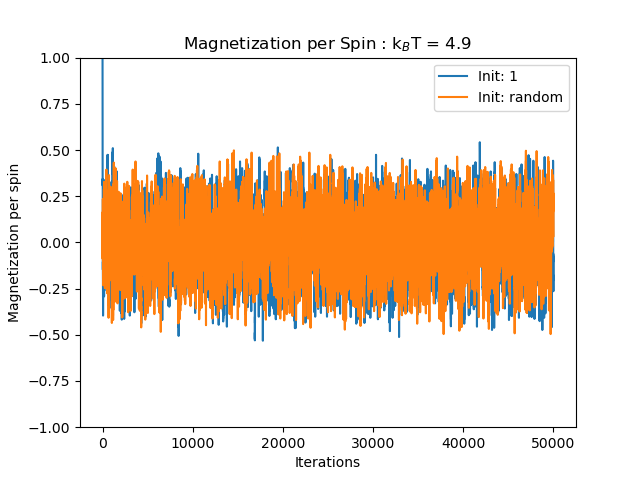
\includegraphics[width=3.7 in]{"../figures/Q3_Magnetization.png"}
\caption{Magnetization per spin at $k_B$T=4.9}
\label{mag4.9}
\end{center}
\end{figure}
\item The instantaneous energy per spin fluctuates around 2.0 at $k_B$T=3.9
\begin{figure}[h]
\begin{center}
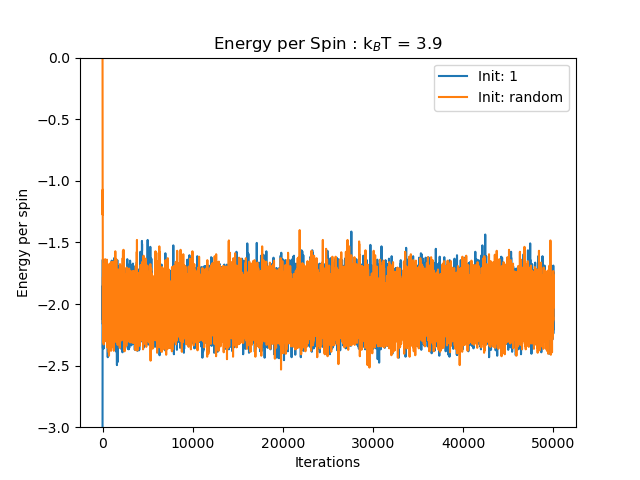
\includegraphics[width=3.7 in]{"../figures/Q4_Energy.png"}
\caption{Energy per spin at $k_B$T=3.9}
\label{energy3.9}
\end{center}
\end{figure}
\item The energy and magnetisation per spin fluctuate about -1.84 and $\pm 0.73$ respectively.
\begin{figure}[h]
\begin{center}
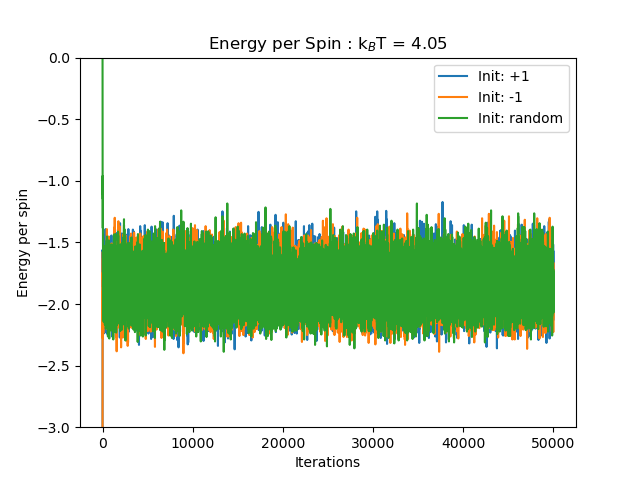
\includegraphics[width=2.8 in]{"../figures/Q5_Energy.png"}
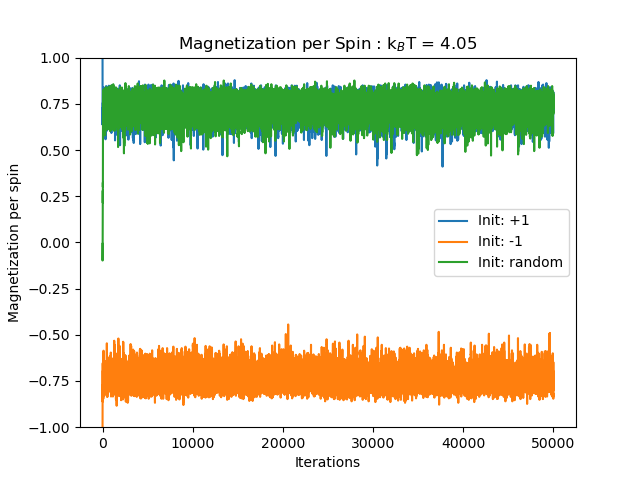
\includegraphics[width=2.8 in]{"../figures/Q5_Magnetization.png"}
\caption{Energy and Magnetization per spin at $k_B$T=4.05}
\label{energymag4.05}
\end{center}
\end{figure}
\item The graphs for Energy and Magnetization at various box sizes have been shown in Figure \ref{enmag39}.
\begin{figure}
\begin{center}
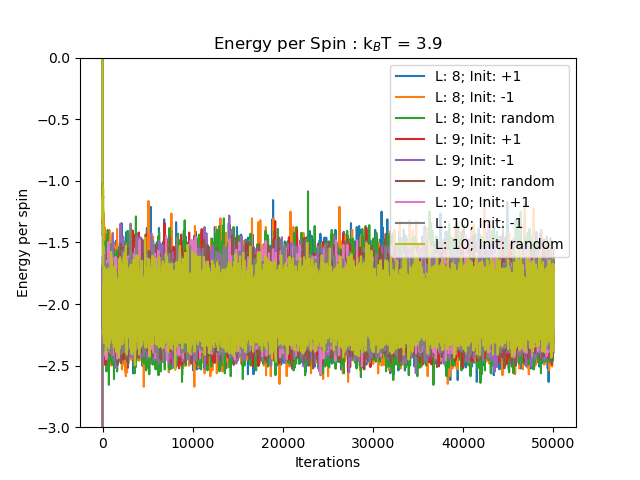
\includegraphics[width=2.8 in]{"../figures/Q6_Energy.png"}
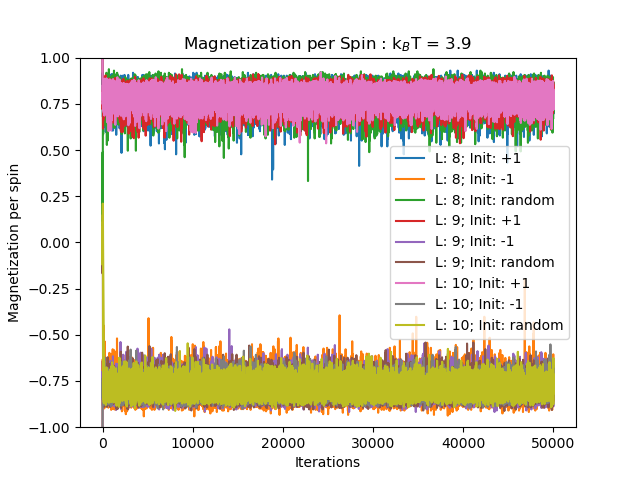
\includegraphics[width=2.8 in]{"../figures/Q6_Magnetization.png"}
\caption{Energy and Magnetization per spin at $k_B$T=3.9}
\label{enmag39}
\end{center}
\end{figure}
\end{enumerate}

The simulation was run as instructed and the following graphs were produced as a result. The magnetisation per spin of the lattice(s) at various temperatures has been plotted in Figure \ref{magtemp}. Likewise, the energy per spin can be seen in Figure \ref{etemp}. The plots for $\chi$ and $C_v$ are in \ref{chi} and \ref{cv} respectively.

\begin{figure}
\begin{center}
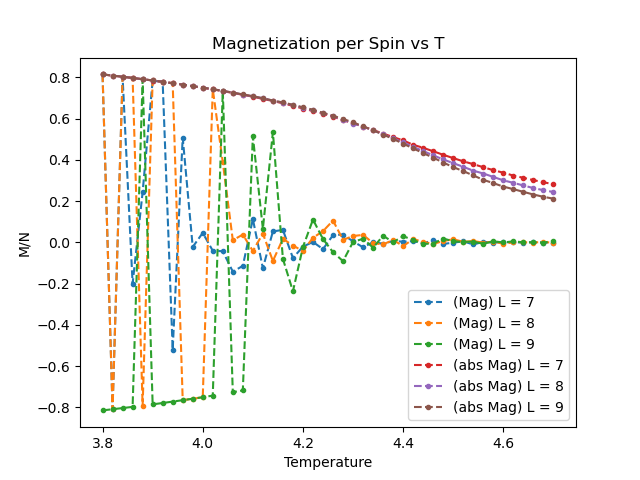
\includegraphics[width=3.0 in]{"../figures/Q7-M.png"}
\caption{Magnetization per spin vs Temperature}
\label{magtemp}
\end{center}
\end{figure}

\begin{figure}
\begin{center}
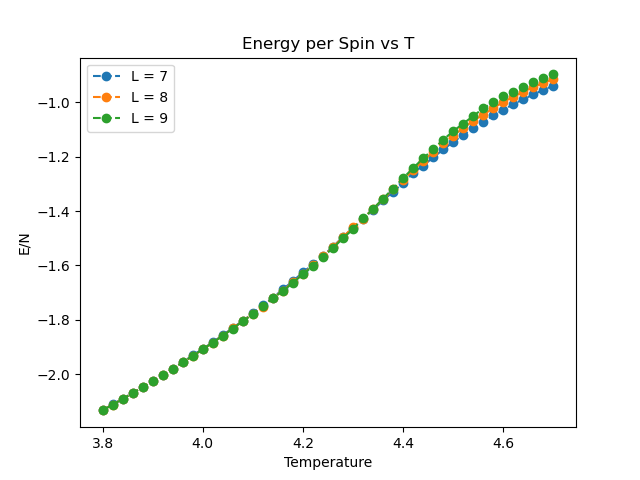
\includegraphics[width=3.0 in]{"../figures/Q7-E.png"}
\caption{Energy per spin vs Temperature}
\label{etemp}
\end{center}
\end{figure}

\begin{enumerate}[resume]
\item The values of $\chi$ at T=4.5 are 932.1, 1835.9 and 3313.7 (in simulation units) for lattice sizes of 7, 8 and 9 respectively.

\item The value fo $C_v$ at peak position for lattice of length 8 is 919.8 (also in simulation units).

\item The value fo $C_v$ at peak position for lattice of length 9 is 1381.7.

\item The magnetization per spin at T = 3.8 for a lattice of length 7 is $\pm 0.814$.

\item The Binder Cumulant plot is shown in Figure \ref{binders}. The point where the curves intersect is T$\approx4.5$.

\item The number of particles jumping from $E_{10}$ to $E_5$ is $10\cdot e^{\Delta E \beta}$ where $\Delta E = E_{5} - E_{10}$ and $\beta = k_BT$.

\begin{figure}
\begin{center}
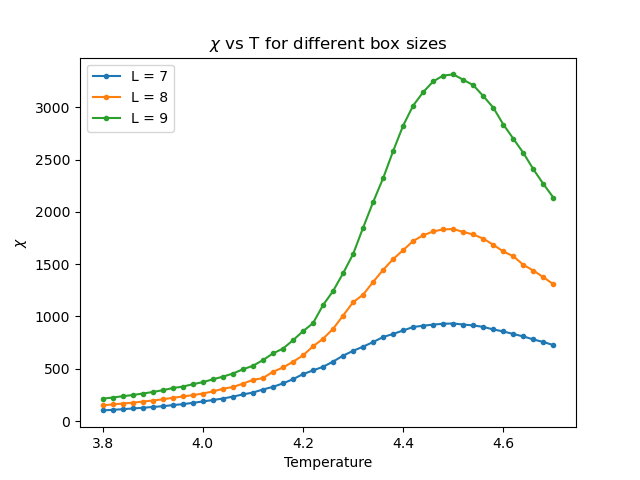
\includegraphics[width=3.0 in]{"../figures/Q7_chi_T.png"}
\caption{$\chi$ vs Temperature}
\label{chi}
\end{center}
\end{figure}
\end{enumerate}

\begin{figure}
\begin{center}
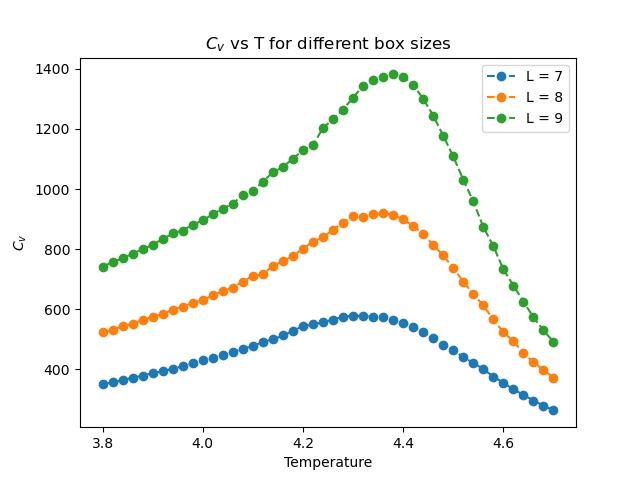
\includegraphics[width=3.0 in]{"../figures/Q7_cv_T.png"}
\caption{$C_v$ vs Temperature}
\label{cv}
\end{center}
\end{figure}
\break
\begin{figure}[!ht]
\begin{center}
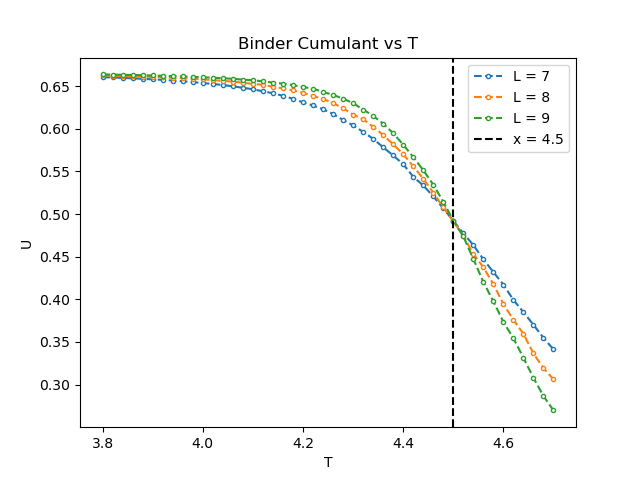
\includegraphics[width=4.0 in]{"../figures/Q11_binder_cumulant.png"}
\caption{Binder Cumulant for different lattice sizes}
\label{binders}
\end{center}
\end{figure}
\end{document}
